%%%%%%%%%%%%%%%%%%%%%%%%%%%%%%%%%%%%%%%%%
% Beamer Presentation
% LaTeX Template
% Version 1.0 (10/11/12)
%
% This template has been downloaded from:
% http://www.LaTeXTemplates.com
%
% License:
% CC BY-NC-SA 3.0 (http://creativecommons.org/licenses/by-nc-sa/3.0/)
%
%%%%%%%%%%%%%%%%%%%%%%%%%%%%%%%%%%%%%%%%%

%----------------------------------------------------------------------------------------
%	PACKAGES AND THEMES
%----------------------------------------------------------------------------------------

\documentclass[UTF8,aspectratio=169,14pt]{ctexbeamer}

\usepackage{hyperref}
\hypersetup{
	colorlinks=true,
	linkcolor=red,
	anchorcolor=blue,
	citecolor=green
}

\mode<presentation> {
	
	% The Beamer class comes with a number of default slide themes
	% which change the colors and layouts of slides. Below this is a list
	% of all the themes, uncomment each in turn to see what they look like.
	
	%\usetheme{default}
	%\usetheme{AnnArbor}
	%\usetheme{Antibes}
	%\usetheme{Bergen}
	%\usetheme{Berkeley}
	%\usetheme{Berlin}
	%\usetheme{Boadilla}
	%\usetheme{CambridgeUS}
	%\usetheme{Copenhagen}
	%\usetheme{Darmstadt}
	%\usetheme{Dresden}
	%\usetheme{Frankfurt}
	%\usetheme{Goettingen}
	%\usetheme{Hannover}
	%\usetheme{Ilmenau}
	%\usetheme{JuanLesPins}
	%\usetheme{Luebeck}
	\usetheme{Madrid}
	%\usetheme{Malmoe}
	%\usetheme{Marburg}
	%\usetheme{Montpellier}
	%\usetheme{PaloAlto}
	%\usetheme{Pittsburgh}
	%\usetheme{Rochester}
	%\usetheme{Singapore}
	%\usetheme{Szeged}
	%\usetheme{Warsaw}
	
	% As well as themes, the Beamer class has a number of color themes
	% for any slide theme. Uncomment each of these in turn to see how it
	% changes the colors of your current slide theme.
	
	%\usecolortheme{albatross}
	%\usecolortheme{beaver}
	%\usecolortheme{beetle}
	%\usecolortheme{crane}
	%\usecolortheme{dolphin}
	%\usecolortheme{dove}
	%\usecolortheme{fly}
	%\usecolortheme{lily}
	%\usecolortheme{orchid}
	%\usecolortheme{rose}
	%\usecolortheme{seagull}
	%\usecolortheme{seahorse}
	%\usecolortheme{whale}
	%\usecolortheme{wolverine}
	
	%\setbeamertemplate{footline} % To remove the footer line in all slides uncomment this line
	%\setbeamertemplate{footline}[page number] % To replace the footer line in all slides with a simple slide count uncomment this line
	
	%\setbeamertemplate{navigation symbols}{} % To remove the navigation symbols from the bottom of all slides uncomment this line
}

\usepackage{graphicx} % Allows including images
\graphicspath{{./figs/}}
\usepackage{booktabs} % Allows the use of \toprule, \midrule and \bottomrule in tables
\usepackage{longtable}
\usepackage{listings}
\usepackage{xcolor}
\lstset{numbers=left, %设置行号位置
	numberstyle=\tiny, %设置行号大小
	keywordstyle=\color{blue}, %设置关键字颜色
	commentstyle=\color[cmyk]{1,0,1,0}, %设置注释颜色
	frame=single, %设置边框格式
	escapeinside=``, %逃逸字符(1左面的键),用于显示中文
	%breaklines, %自动折行
	extendedchars=false, %解决代码跨页时,章节标题,页眉等汉字不显示的问题
	xleftmargin=2em,xrightmargin=2em, aboveskip=1em, %设置边距
	tabsize=4, %设置tab空格数
	showspaces=false %不显示空格
}
% Fonts
% \usepackage{libertine}
% \setmonofont{Courier}
\setCJKsansfont[ItalicFont=Noto Serif CJK SC Black, BoldFont=Noto Sans CJK SC Black]{Noto Sans CJK SC}

%\def\imagepath{./resources/graphics}
%\usepackage[imagepath=\imagepath]{ditaa}
%\graphicspath{ {\imagepath/} }


%\usepackage{pgfpages}
%\setbeameroption{show notes on second screen}
%%----------------------------------------------------------------------------------------
%	TITLE PAGE
%----------------------------------------------------------------------------------------

\title[第9讲]{第九讲 :进程、线程和协程} % The short title appears at the bottom of every slide, the full title is only on the title page
\subtitle{第3节:协程(coroutine)}
\author{向勇、陈渝、李国良} % Your name
\institute[清华大学] % Your institution as it will appear on the bottom of every slide, may be shorthand to save space
{
	清华大学计算机系 \\ % Your institution for the title page
	\medskip
	\textit{xyong,yuchen,liguoliang@tsinghua.edu.cn} % Your email address
}
\date{\today} % Date, can be changed to a custom date


\begin{document}

\begin{frame}
\titlepage % Print the title page as the first slide
\end{frame}

%----------------------------------------------
\begin{frame}
\frametitle{提纲} % Table of contents slide, comment this block out to remove it
\tableofcontents % Throughout your presentation, if you choose to use \section{} and \subsection{} commands, these will automatically be printed on this slide as an overview of your presentation
\end{frame}
%----------------------------------------------
%%	PRESENTATION SLIDES
%----------------------------------------------
%------------------------------------------------
\section{第2节:用户线程的实现}% Sections can be created in order to organize your presentation into discrete blocks, all sections and subsections are automatically printed in the table of contents as an overview of the talk
% 
% 参考文献:
    \begin{itemize}
        \item \href{https://cfsamson.gitbook.io/green-threads-explained-in-200-lines-of-rust/}{Green Threads Explained in 200 Lines of Rust...}
        \item \href{https://github.com/cfsamson/example-greenthreads}{完整源代码}
        \item 知乎上的中文版本:\href{https://zhuanlan.zhihu.com/p/101061389}{两百行Rust代码解析绿色线程原理(四)一个绿色线程的实现}
    \end{itemize}
% 
\end{frame}
%------------------------------------------------
\subsection{线程与CPU架构}
% 
%------------------------------------------------
\begin{frame}[fragile]
    \frametitle{CPU体系结构}
% 
% 用户线程调度是非抢占式的;
% 
% CPU体系结构:通用寄存器
% 
% 出处:\href{https://software.intel.com/content/www/us/en/develop/articles/intel-sdm.html\#combined}{Combined Volume Set of Intel® 64 and IA-32 Architectures Software Developer’s Manuals}、\href{https://software.intel.com/content/dam/develop/external/us/en/documents-tps/325462-sdm-vol-1-2abcd-3abcd.pdf}{325462-sdm-vol-1-2abcd-3abcd.pdf} P76 Figure 3-4. General System and Application Programming Registers
% 
	\begin{figure}
		\centering
		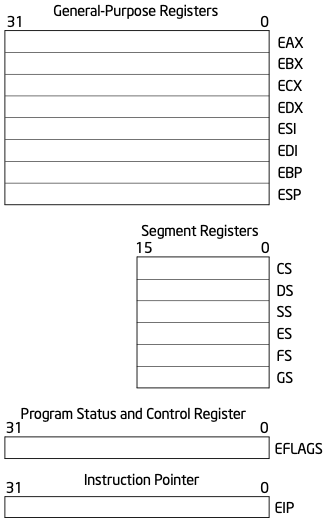
\includegraphics[width=0.5\linewidth]{figs/x86-32-registers.png}
		\caption{x86-32-registers}
	\end{figure}


% 
% 出处:\href{https://software.intel.com/content/dam/develop/external/us/en/documents-tps/325462-sdm-vol-1-2abcd-3abcd.pdf}{325462-sdm-vol-1-2abcd-3abcd.pdf} P77 Table 3-2. Addressable General Purpose Registers
% 
	\begin{figure}
		\centering
		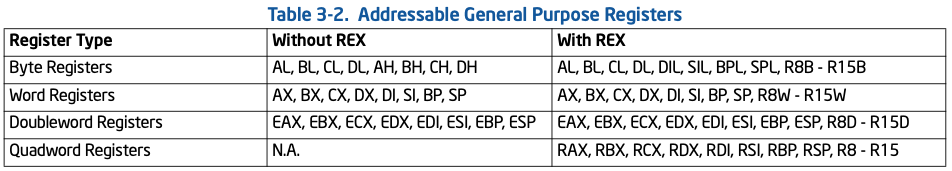
\includegraphics[width=0.5\linewidth]{figs/8-16-32-64-registers.png}
		\caption{8-16-32-64-registers}
	\end{figure}


% 
\end{frame}
%------------------------------------------------
\begin{frame}[fragile]
    \frametitle{X86汇编语言}
% 
	\begin{figure}
		\centering
		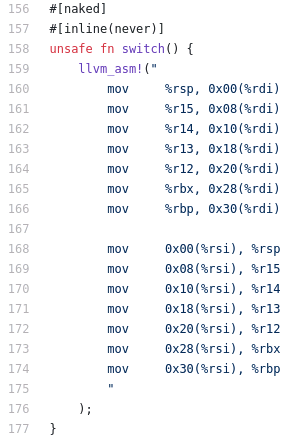
\includegraphics[width=0.5\linewidth]{figs/green-thread-switch.png}
		\caption{green-thread-switch}
	\end{figure}


% 
\end{frame}
%------------------------------------------------
\subsection{线程上下文和线程栈}
%------------------------------------------------
\begin{frame}[fragile]
    \frametitle{线程上下文\href{https://github.com/cfsamson/example-greenthreads/blob/master/src/main.rs\#L28}{数据结构}`ThreadContext`}
% 
	\begin{figure}
		\centering
		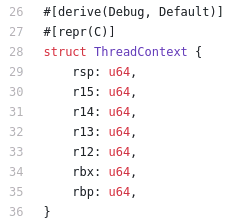
\includegraphics[width=0.5\linewidth]{figs/green-thread-ThreadContext.png}
		\caption{green-thread-ThreadContext}
	\end{figure}


% 
\end{frame}
%------------------------------------------------
\begin{frame}[fragile]
    \frametitle{栈空间大小}
    \begin{itemize}
        \item 现代操作系统中启动进程时,标准栈大小通常为8MB;
        \item 可能出现“栈溢出”;
        \item 当我们自己控制栈时,我们可以选择我们想要的大小;
        \item 可增长栈:当栈空间用完时,会分配一个更大的栈并将栈内容移到更大的栈上,并恢复程序继续执行,不会导致栈溢出;(Go 语言)
    \end{itemize}
% 
% 
% 
\end{frame}
%------------------------------------------------
\begin{frame}[fragile]
    \frametitle{栈布局}
% 
% 出处:\href{https://software.intel.com/content/dam/develop/external/us/en/documents-tps/325462-sdm-vol-1-2abcd-3abcd.pdf}{325462-sdm-vol-1-2abcd-3abcd.pdf} P152 Figure 6-1. Stack Structure
% 
	\begin{figure}
		\centering
		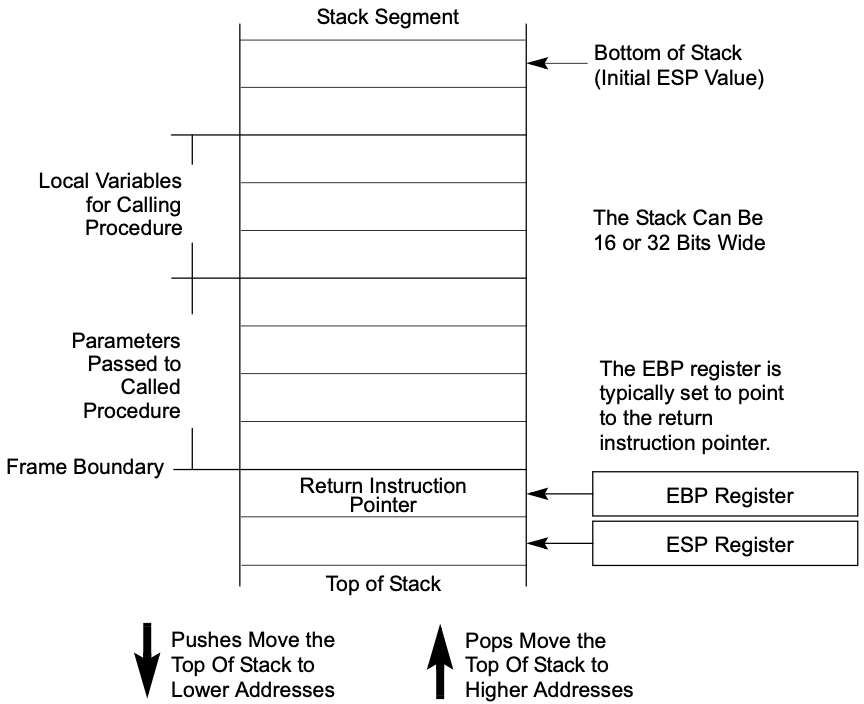
\includegraphics[width=0.5\linewidth]{figs/stack-structure.png}
		\caption{stack-structure}
	\end{figure}


% 
% 
% 
\end{frame}
%------------------------------------------------
\subsection{线程控制块和运行时支持}
%------------------------------------------------
\begin{frame}[fragile]
    \frametitle{线程控制块\href{https://github.com/cfsamson/example-greenthreads/blob/master/src/main.rs\#L19}{数据结构}`Thread`}
% 
% \href{https://docs.microsoft.com/zh-cn/cpp/c-language/naked-functions?view=msvc-160}{裸函数}naked_functions:为了与编译器协调处理函数调用和中断处理中栈的使用,而定义的一个约定。它仅影响函数的 prolog 和 epilog 序列的编译器代码生成的性质。
% 
	\begin{figure}
		\centering
		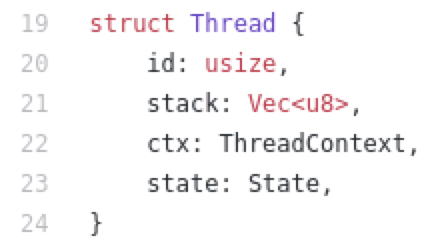
\includegraphics[width=0.5\linewidth]{figs/thread.png}
		\caption{thread}
	\end{figure}


% 
\end{frame}
%------------------------------------------------
\begin{frame}[fragile]
    \frametitle{线程\href{https://github.com/cfsamson/example-greenthreads/blob/master/src/main.rs\#L49}{运行时}支持`Runtime`}
% 
% new
% run
% t_return
% t_yield
% 
\end{frame}
%------------------------------------------------
\subsection{用户线程API和线程切换}
%------------------------------------------------
\begin{frame}[fragile]
    \frametitle{\href{https://github.com/cfsamson/example-greenthreads/blob/master/src/main.rs\#L119}{线程API}:`spawn`}
% 
	\begin{figure}
		\centering
		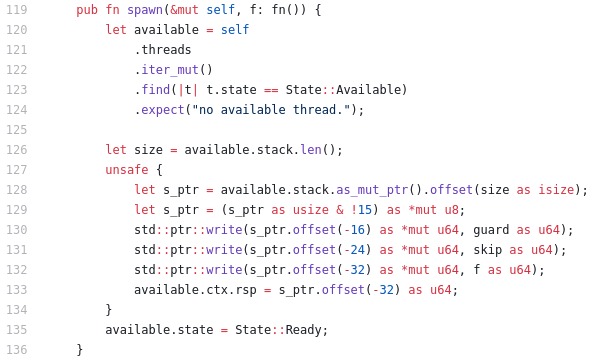
\includegraphics[width=0.5\linewidth]{figs/spawn.png}
		\caption{spawn}
	\end{figure}


% 
\end{frame}
%------------------------------------------------
\begin{frame}[fragile]
    \frametitle{\href{https://github.com/cfsamson/example-greenthreads/blob/master/src/main.rs\#L119}{线程API}:yield_thread}
% 
	\begin{figure}
		\centering
		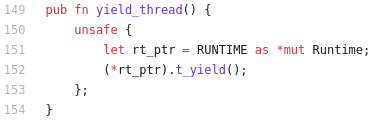
\includegraphics[width=0.5\linewidth]{figs/yield_thread.png}
		\caption{yield_thread}
	\end{figure}


% 
\end{frame}
%------------------------------------------------
\begin{frame}[fragile]
    \frametitle{\href{https://github.com/cfsamson/example-greenthreads/blob/master/src/main.rs\#L158}{线程切换}`switch`}
% 
	\begin{figure}
		\centering
		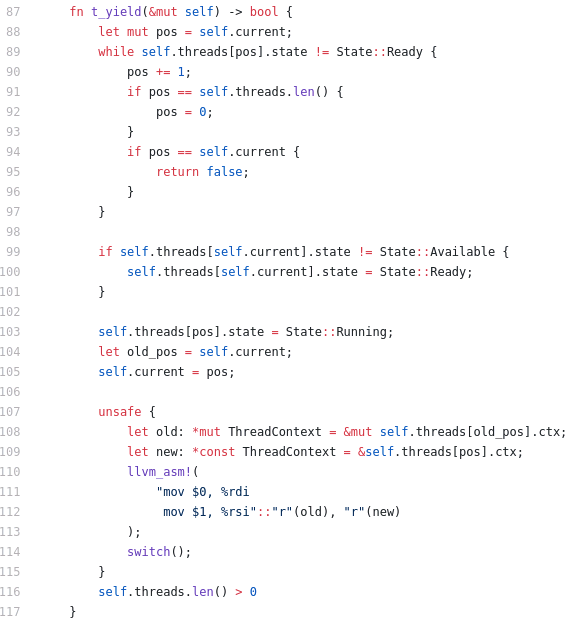
\includegraphics[width=0.5\linewidth]{figs/t_yield.png}
		\caption{t_yield}
	\end{figure}


% 
% 用户线程的操作系统依赖:示例适用于 OSX、Linux 和 Windows
\end{frame}
%------------------------------------------------
\end{document}
